%!TEX root = ../dissertation.tex
%\begin{savequote}[75mm]
%Nulla facilisi. In vel sem. Morbi id urna in diam dignissim feugiat. Proin molestie %tortor eu velit. Aliquam erat volutpat. Nullam ultrices, diam tempus vulputate egestas, %eros pede varius leo.
%\qauthor{Quoteauthor Lastname}
%\end{savequote}

\chapter{Algorithms}
\label{algorithms}

At this point, the dataset is ready for the algorithms development. Recalling that the dataset is composed by comments labeled according to some identified topics, with a three sentiment polarity degrees, plus an additional relevancy flag, that makes the final problem a four-labels classification task. This problem has been faced in different ways, that will be explained in the Chapter \ref{experiments}. In this Chapter, will be argued the algorithms that will be involved in the classifications and the choices made for the development. The main pipeline remain the same of state of the art text classification problems, that has been presented in Chapter \ref{state-of-the-art}, but some implementation choices are needed in order to make the algorithms specific for the automotive domain. Since (almost) same algorithms can be run on different datasets, it has been made a comparison using the Twitter's Airline dataset, and the differences on implementation have been explained later on.\\
All code has been developed in Python 3.7 (\url{https://www.python.org/downloads/release/python-370/}) using the Jupyter Notebook (\url{https://jupyter.org/}), that is a web application that allows to create live Python code. 
%The code is available on the repository \url{https://github.com/elRava/master_thesis_sentiment_analysis/}.
%% TODO dare occhiata se tenere link repo


\section{SVM and Logistic Regression Classification}

The simpler algorithms implemented in this work, follow the state of the art pipeline for text classification. Since the algorithms are supposed to work on very different environments, they present some differences, especially on preprocessing stage. The same algorithm is used for both binary classification for relevance test, and multilabel sentiment classification.\\


\subsection{Twitter Preprocessing}

Preprocessing for Twitter's dataset handles Twitter's specific tokens and normalize them in order to treat them in a standard way. Some functions are optional in the sense that the preprocessing has been made parametric and it is possible to choose if do them or not. The steps are the followings:

\begin{itemize}
	\item Transformation text to lowercase;
	\item Replace two or more dots with space, in order to remove useless punctuation;
	\item For every token, remove spaces, " and ';
	\item Optional substitution of the URLs with "URL";
	\item Optional replacing user mentions (@user) with "USER\_MENTION";
	\item Optional removing "\#" from hashtags (\#hashtag);
	\item Optional removing retweet character ("RT");
	\item Optional grouping emoticons into positive and negative ones and replacing them with "EMO\_POS" and "EMO\_NEG". Positive emoticons are: :), : ), :-), (:, ( :, (-:, :'), :D, : D, :-D, xD, x-D, XD, X-D, <3, :*, ;-), ;), ;-D, ;D, (;,  (-;, while Negative ones are: :-(, : (, :(, ):, )-:, :,(, :'(, :"( ;
	\item Removing residual multiple spaces.
\end{itemize}



\subsection{Italian Automotive Dataset Preprocessing}

As in Twitter's preprocessing, the goal is to reduce noise by handling domain specific terms. Also in this case the preprocessing has been made parametric. The steps are the followings:

\begin{itemize}
	\item Encoding correction;
	\item Punctuation removal;
	\item Transformation text to lowercase;
	\item Removal of character repetitions: keep at maximum three consecutive character repeated;
	\item Replaced question marks and consecutive question marks with respectively "QMARK" and "MULTI\_QMARK";
	\item Replaced exclamation marks and consecutive question marks with respectively "EMARK" and "MULTI\_EMARK";
	\item Replacing URLs with "URL";
	\item Replacing HTML picture tags with "IMG";
	\item Stopwords removal;
	\item Optional replacing brands with "BRAND" and car models with "MODEL": since the classifications are considered brand independent, it comes the idea of replacing all brand names with a common token. The dictionary of all manufacturers and models has been scraped from \url{https://www.auto-data.net}, since a complete one has not be found;
	\item Replacing speed metrics with "SPEED": since the car independent intentions, it does not matter the actual speed values, for instance 150 km/h may be good for a city car, but not so good for a sport car. Moreover, it depends on the context, so the decision of ignore the numerical value. For the same reason also consumption metrics have been replaced with "CONSUMPTION", weights metrics with "WEIGHT" and power metrics with "POWER";
	\item Replaced distances with "DISTANCE";
	\item Replaced numbers with three or more digits with "NUMBER".
\end{itemize}

All operation have been implemented exploiting regular expressions from the re library (\url{https://github.com/python/cpython/blob/3.7/Lib/re.py}) and common natural language processing operation from nltk library (\url{https://www.nltk.org/}).

After preprocessing, it has been adopted the "snowball" stemmer from nltk library (\url{https://www.nltk.org/_modules/nltk/stem/snowball.html}), for normalization purposes.


\subsection{Classification}

Following the preprocessing, it is applied the stemmer. The result of the whole preprocessing phase on a tweet is:

\begin{description}
	\item \textit{@united I do not see where it talks about military baggage fees. Can you please guide me. Thanks}
	\item \textit{USER\_MENTION see talk militari baggag fee  pleas guid  thank
	}
\end{description}

and on the Italian automotive dataset is:

\begin{description}
	\item \textit{Sono reali calcolati nel arco del tutto anno nel estate qualcosa in più causa gomme di 17" e climatizzatore nel inverno un po di meno. Per quanto riguarda le autostrade quelle che percorro io principalmente la A4 e molto congestionata cosi spesso la media e 110-115 km/h che ovviamente influisce positivamente a i consumi. Ma quello che mi piace di più è assenza dei guasti. Sulla vecchia Accord il primo guasto lo ho avuto a 200000 km si è rotto il termostato della clima. Ogni tanto faccio giro di altri forum e leggo delle turbine rotte catene di distribuzione progettate male iniettori fatti male mah nel 2015 per me sono le cose incomprensibili . Con tutti gli difetti che può avere preferisco la Honda. }
	
	\item \textit{real calcol arco anno MODEL qualcos caus gomm MODEL climatizz invern po men riguard autostrad percorr principal MODEL molt congestion cos spess med MODEL SPEED ovvi influ posit consum piac assenz guast vecc MODEL prim guast DISTANCE rott termost clim ogni MODEL gir altri forum legg turbin rott caten distribu progett mal iniettor fatt mal mah NUMBER me cos incomprens difett può aver prefer BRAND}
\end{description}

For all experiments on the Italian automotive dataset, we firstly focused on just one topic, then the same procedure has been extended to all others. Since this dataset has not just one text, but it contain also the quote, the classification should involve both texts. It has been implemented joining the texts and, in a parametric way, adding a suffix to each word like "\_TEXT" or "\_QUOTE" weather a word is belonging to the text or to the quote.

For vectorization it has been chosen the \ac{TFIDF} method considering both unigrams and bigrams. Classification involved either Support Vector Machine classificator and Logistic Regression classificator for different experiments, both from scikit-learn library (\url{https://scikit-learn.org/}).


An important task for model selection consists on hyperparameters optimization. Hyperparameters are model parameters that must be chosen before the learning process begins. In general, different algorithms require different hyperparameters, and some others none. The search of the optimum parameters has been implemented using a grid search, which requires a proper list of parameters and a list of testing values. It searches among all the parameters, the ones that, when the model is trained with those, reaches the best score. The reference score, of course, must be defined previously and depends on the classification problem.
Feature selection has been performed in the same way for both SVM and Logistic Regression. After a first optimization involving all features, found weights of the classifier are ranked with respect to the absolute value. Then, after some tries it is defined an adequate cutoff value which selects the features to keep. From scikit-learn library it is possible to achieve the weights of the binary classifiers that compose the one-versus-one multiclass classifier, so for a three-labels classifier, there are three sets of weights. From the different sets, the goal is to find the most relevant features for all binary classifiers, from here the choice to act in this way: for every set of weights, apply the cutoff to select the most important features in the binary case, and then make the union of all sets of selected features in order to have just one set of features for every classifier.



 The final model is obtained by train again the algorithm keeping only the selected features.


\section{BPEF Revisitation}

The second algorithm employed for text classification is a revisitation of the BPEF algorithm described in Chapter \ref{state-of-the-art}. It has been chosen this algorithm because of its proved good performance and stability in Twitter sentiment analysis, and above all, the capability to adaptation to slightly different problems. The adaptation procedure will be described in the followings paragraphs.

\subsection{Parametric Model}

As shown in Section 2.4.1, Bootstrap Ensemble Framework is based upon a parametric model that involves dataset, feature and classifier parameters. Every type of parameters had been modified from the original paper and it has been adapted for the problem of this work.

\subsubsection{Dataset Parameters}

In the original BPEF algorithm, the target dataset was integrated with other dataset of similar domain. The purpose was to enrich the dictionary of common saying and common patterns that are used for sentiment classification in order to make the classifier more stable. Actually, the Italian automotive dataset already contains a comments with a large variety of expressions, and most important, it can be considered also an union of different datasets, in fact it contain comments from very different car brands, that cause variety on subjects and patterns. For instance, suppose that the target classification is a the set of comments of sports cars, but since the dataset contain comments of every type of automotive vehicles, then off-topic ones can be considered as an integration, that in BPEF algorithm consisted in the aggregation of multiple datasets. In conclusion, because of these reasons, dataset parameters have just been removed.


\subsubsection{Feature Parameters}

% word, pos, pos+word, swnt
% io ho fatto word, pos, swnt
As described in Chapter 2.4.1, with BPEF algorithm every sentence is processed in four parallel ways, defined by the feature parameters that are: "word", "POS", "semantic" and "SWNt". For semplicity and lack of Italian resources, in the BPEF revisitation have been implemented "word", "POS" and "SWNt" features. For POS features it was exploited Python's "spacy" library (\url{https://spacy.io/models/it}) that also supports Italian, while for what  concerns words' sentiment polarities, SentiWordNet does not support Italian, so it has been utilized "OpeNER" (\url{https://dspace-clarin-it.ilc.cnr.it/repository/xmlui/handle/20.500.11752/ILC-73}) that is a list of words that has been semi-automatically labeled with ItalWordNet v.2, starting from a list of 1000 manually labeled words.\\
On top of these features groups, it has been applied the words summarizing that has been presented in Section 4.1.2. Finally, the stemmer is applied for normalization.\\
An example of the different preprocessings is:

\begin{description}
	\item[Original]: \textit{Sono reali calcolati nel arco del tutto anno nel estate qualcosa in più causa gomme di 17" e climatizzatore nel inverno un po di meno. Per quanto riguarda le autostrade quelle che percorro io principalmente la A4 e molto congestionata cosi spesso la media e 110-115 km/h che ovviamente influisce positivamente a i consumi. Ma quello che mi piace di più è assenza dei guasti. Sulla vecchia Accord il primo guasto lo ho avuto a 200000 km si è rotto il termostato della clima. Ogni tanto faccio giro di altri forum e leggo delle turbine rotte catene di distribuzione progettate male iniettori fatti male mah nel 2015 per me sono le cose incomprensibili . Con tutti gli difetti che può avere preferisco la Honda.};
	\item[word]: \textit{real calcol arco anno MODEL qualcos caus gomm MODEL climatizz invern po men riguard autostrad percorr principal MODEL molt congestion cos spess med MODEL SPEED ovvi influ posit consum piac assenz guast vecc MODEL prim guast DISTANCE rott termost clim ogni MODEL gir altri forum legg turbin rott caten distribu progett mal iniettor fatt mal mah NUMBER me cos incomprens difett può aver prefer BRAND};
	\item[SWNt]: \textit{POS\_2 calcolati NEU\_2 anno MODEL qualcosa POS\_5 gomme MODEL climatizzatore inverno po meno riguarda autostrade percorro principalmente MODEL molto congestionata cosi spesso NEU\_2 MODEL SPEED ovviamente influisce POS\_10 consumi piace NEG\_6 guasti vecchia MODEL POS\_6 NEG\_5 DISTANCE NEG\_5 termostato clima ogni MODEL NEU\_2 altri forum leggo turbine rotte catene NEU\_5 progettate NEG\_6 iniettori fatti NEG\_6 mah NUMBER me cose incomprensibili difetti può NEG\_5 preferisco BRAND};
	\item[POS]: \textit{ADJ VERB ADJ NOUN PROPN PRON NOUN ADJ PROPN NOUN ADJ VERB ADV VERB NOUN ADJ ADV PROPN ADV VERB ADJ ADV ADJ PROPN PROPN ADV VERB ADV NOUN VERB NOUN NOUN VERB PROPN ADJ NOUN PROPN VERB ADJ NOUN DET PROPN NOUN DET NOUN DET NOUN VERB VERB NOUN VERB ADV NOUN VERB ADV NOUN PROPN PRON NOUN ADJ NOUN AUX VERB NOUN PROPN adj\_real verb\_calcol adj\_arc noun\_ann PROPN\_MODEL pron\_qualc noun\_caus adj\_gomm PROPN\_MODEL noun\_climatizz adj\_invern verb\_p adv\_men verb\_riguard noun\_autostrad adj\_percorr adv\_principal PROPN\_MODEL adv\_molt verb\_congestion adj\_cos adv\_spess adj\_med PROPN\_MODEL PROPN\_SPEED adv\_ovv verb\_influ adv\_posit noun\_consum verb\_piac noun\_asst noun\_guast verb\_vecc PROPN\_MODEL adj\_prim noun\_guast PROPN\_DISTANCE verb\_rott adj\_termost noun\_clim det\_ogn PROPN\_MODEL noun\_gir det\_altr noun\_forum det\_legg noun\_turbin verb\_rott verb\_caten noun\_distribu verb\_progett adv\_mal noun\_iniettor verb\_fatt adv\_mal noun\_mah PROPN\_NUMBER pron\_m noun\_cos adj\_incomprens noun\_difett aux\_pu verb\_av noun\_prefer PROPN\_BRAND} 
\end{description}


\subsubsection{Classifier Parameters}

In the learning stack are included some commonly used classification algorithms: \acl{SVM}, Logistic Regression, Na{\"i}ve Bayes and Random Forest, that work in an ensemble, making the model more stable.


\subsubsection{Contraction: Step-Wise Model Selection}

Original BPEF model essentially consists in an ensemble model, made by a number of classifiers that is the product of dataset, features and classification parameters. Since in the original paper this number was excessive, it was applied the Step-wise Iterative Model Selection, that is an heuristic iterative algorithm used for selecting the best subset of classifiers. In this work the number of classifiers is not so high, in fact there are no dataset parameters, 6 feature parameters ("word", "POS" and "SWNt" with and without words summarizing) and 4 classifier parameters, counting a total of 24 models, so the selection is not implemented.

\subsection{Classification}

In BPEF model, features selection is performed using Information Gain (IG) heuristic, and must be necessary applied before classification, since it is based upon probability characteristics of the dataset, rather than classifiers' weights. IG features selection has been implemented using "info-gain" library (\url{https://pypi.org/project/info-gain/}), that is based on discrete probability distributions, so the vectorization consisted on Term Frequency, instead of TF-IDF, considering both unigrams and bigrams. Feature selection consisted into ranking all features based on their IG, and then selecting a reasonable cutoff value that eliminates the feature with lower IG.\\
For every classifier it is necessary the hyperparameters optimization process, that has been implemented with a grid search, where each model validation is performed with a 5-folds cross validation, searching for the model that gives the best score.


\section{Cascade Classification}

A text classifier can be used for all relevance classification, sentiment classification and for the whole four-labels classification. In this way the dual goal of classification, that is the topic detection and sentiment classification, can be faced in two different ways: a one-step classification with a 4-labels classifier (Figure \ref{fig:4label-class}), or a two-steps one with a cascade classifier (Figure \ref{fig:cascade-class}). The second option consists in a cascade of two classifiers, where the first one deals with relevance targeting, while the second one with the sentiment classification. This may improve the final performance because both classifiers are thought for different purposes, while having only one model may have difficulties on both topic relevance and sentiment.


\begin{figure}[ht]
	\centering
	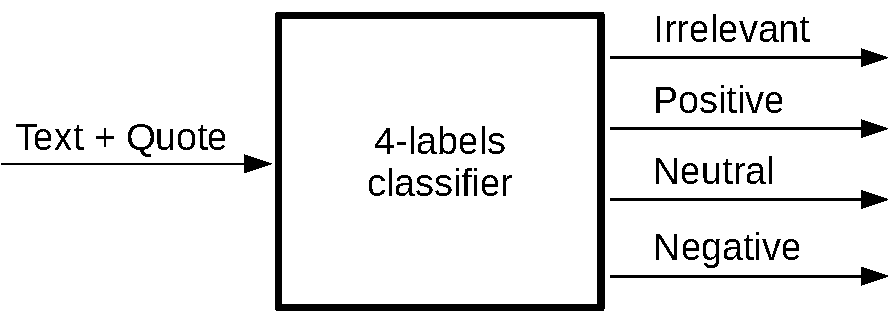
\includegraphics[width=0.7\textwidth]{figures/draw/blocks_class.pdf}
	\caption{4-labels classifier}
	\label{fig:4label-class}
\end{figure}

\begin{figure}[ht]
	\centering
	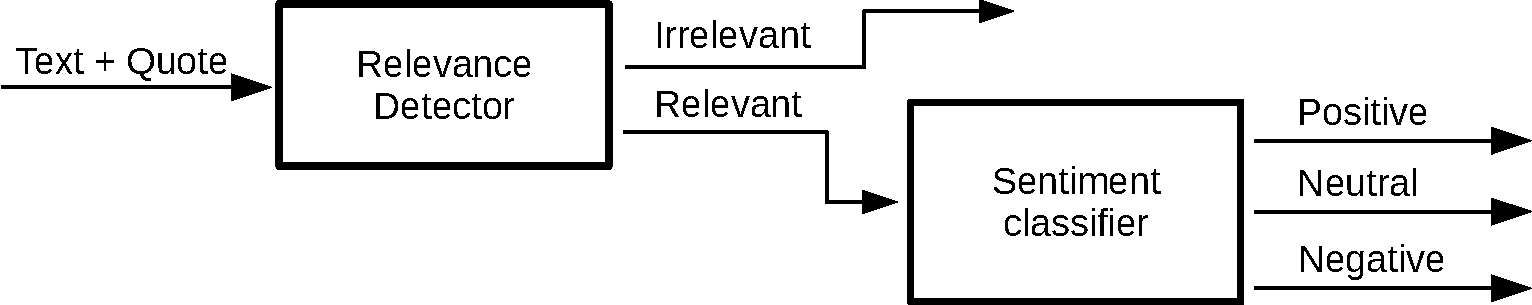
\includegraphics[width=1\textwidth]{figures/draw/blocks_cascade.pdf}
	\caption{Cascade classifier}
	\label{fig:cascade-class}
\end{figure}











% tsa svm
% tsa bpef
% my svm rel
% my logreg rel
% my svm snt
% my svm 4lab
% my bpef snt
% my cascade logreg svm
%my cascade logreg bpef



